\documentclass[1p]{elsarticle_modified}
%\bibliographystyle{elsarticle-num}

%\usepackage[colorlinks]{hyperref}
%\usepackage{abbrmath_seonhwa} %\Abb, \Ascr, \Acal ,\Abf, \Afrak
\usepackage{amsfonts}
\usepackage{amssymb}
\usepackage{amsmath}
\usepackage{amsthm}
\usepackage{scalefnt}
\usepackage{amsbsy}
\usepackage{kotex}
\usepackage{caption}
\usepackage{subfig}
\usepackage{color}
\usepackage{graphicx}
\usepackage{xcolor} %% white, black, red, green, blue, cyan, magenta, yellow
\usepackage{float}
\usepackage{setspace}
\usepackage{hyperref}

\usepackage{tikz}
\usetikzlibrary{arrows}

\usepackage{multirow}
\usepackage{array} % fixed length table
\usepackage{hhline}

%%%%%%%%%%%%%%%%%%%%%
\makeatletter
\renewcommand*\env@matrix[1][\arraystretch]{%
	\edef\arraystretch{#1}%
	\hskip -\arraycolsep
	\let\@ifnextchar\new@ifnextchar
	\array{*\c@MaxMatrixCols c}}
\makeatother %https://tex.stackexchange.com/questions/14071/how-can-i-increase-the-line-spacing-in-a-matrix
%%%%%%%%%%%%%%%

\usepackage[normalem]{ulem}

\newcommand{\msout}[1]{\ifmmode\text{\sout{\ensuremath{#1}}}\else\sout{#1}\fi}
%SOURCE: \msout is \stkout macro in https://tex.stackexchange.com/questions/20609/strikeout-in-math-mode

\newcommand{\cancel}[1]{
	\ifmmode
	{\color{red}\msout{#1}}
	\else
	{\color{red}\sout{#1}}
	\fi
}

\newcommand{\add}[1]{
	{\color{blue}\uwave{#1}}
}

\newcommand{\replace}[2]{
	\ifmmode
	{\color{red}\msout{#1}}{\color{blue}\uwave{#2}}
	\else
	{\color{red}\sout{#1}}{\color{blue}\uwave{#2}}
	\fi
}

\newcommand{\Sol}{\mathcal{S}} %segment
\newcommand{\D}{D} %diagram
\newcommand{\A}{\mathcal{A}} %arc


%%%%%%%%%%%%%%%%%%%%%%%%%%%%%5 test

\def\sl{\operatorname{\textup{SL}}(2,\Cbb)}
\def\psl{\operatorname{\textup{PSL}}(2,\Cbb)}
\def\quan{\mkern 1mu \triangleright \mkern 1mu}

\theoremstyle{definition}
\newtheorem{thm}{Theorem}[section]
\newtheorem{prop}[thm]{Proposition}
\newtheorem{lem}[thm]{Lemma}
\newtheorem{ques}[thm]{Question}
\newtheorem{cor}[thm]{Corollary}
\newtheorem{defn}[thm]{Definition}
\newtheorem{exam}[thm]{Example}
\newtheorem{rmk}[thm]{Remark}
\newtheorem{alg}[thm]{Algorithm}

\newcommand{\I}{\sqrt{-1}}
\begin{document}

%\begin{frontmatter}
%
%\title{Boundary parabolic representations of knots up to 8 crossings}
%
%%% Group authors per affiliation:
%\author{Yunhi Cho} 
%\address{Department of Mathematics, University of Seoul, Seoul, Korea}
%\ead{yhcho@uos.ac.kr}
%
%
%\author{Seonhwa Kim} %\fnref{s_kim}}
%\address{Center for Geometry and Physics, Institute for Basic Science, Pohang, 37673, Korea}
%\ead{ryeona17@ibs.re.kr}
%
%\author{Hyuk Kim}
%\address{Department of Mathematical Sciences, Seoul National University, Seoul 08826, Korea}
%\ead{hyukkim@snu.ac.kr}
%
%\author{Seokbeom Yoon}
%\address{Department of Mathematical Sciences, Seoul National University, Seoul, 08826,  Korea}
%\ead{sbyoon15@snu.ac.kr}
%
%\begin{abstract}
%We find all boundary parabolic representation of knots up to 8 crossings.
%
%\end{abstract}
%\begin{keyword}
%    \MSC[2010] 57M25 
%\end{keyword}
%
%\end{frontmatter}

%\linenumbers
%\tableofcontents
%
\newcommand\colored[1]{\textcolor{white}{\rule[-0.35ex]{0.8em}{1.4ex}}\kern-0.8em\color{red} #1}%
%\newcommand\colored[1]{\textcolor{white}{ #1}\kern-2.17ex	\textcolor{white}{ #1}\kern-1.81ex	\textcolor{white}{ #1}\kern-2.15ex\color{red}#1	}

{\Large $\underline{12n_{0108}~(K12n_{0108})}$}

\setlength{\tabcolsep}{10pt}
\renewcommand{\arraystretch}{1.6}
\vspace{1cm}\begin{tabular}{m{100pt}>{\centering\arraybackslash}m{274pt}}
\multirow{5}{120pt}{
	\centering
	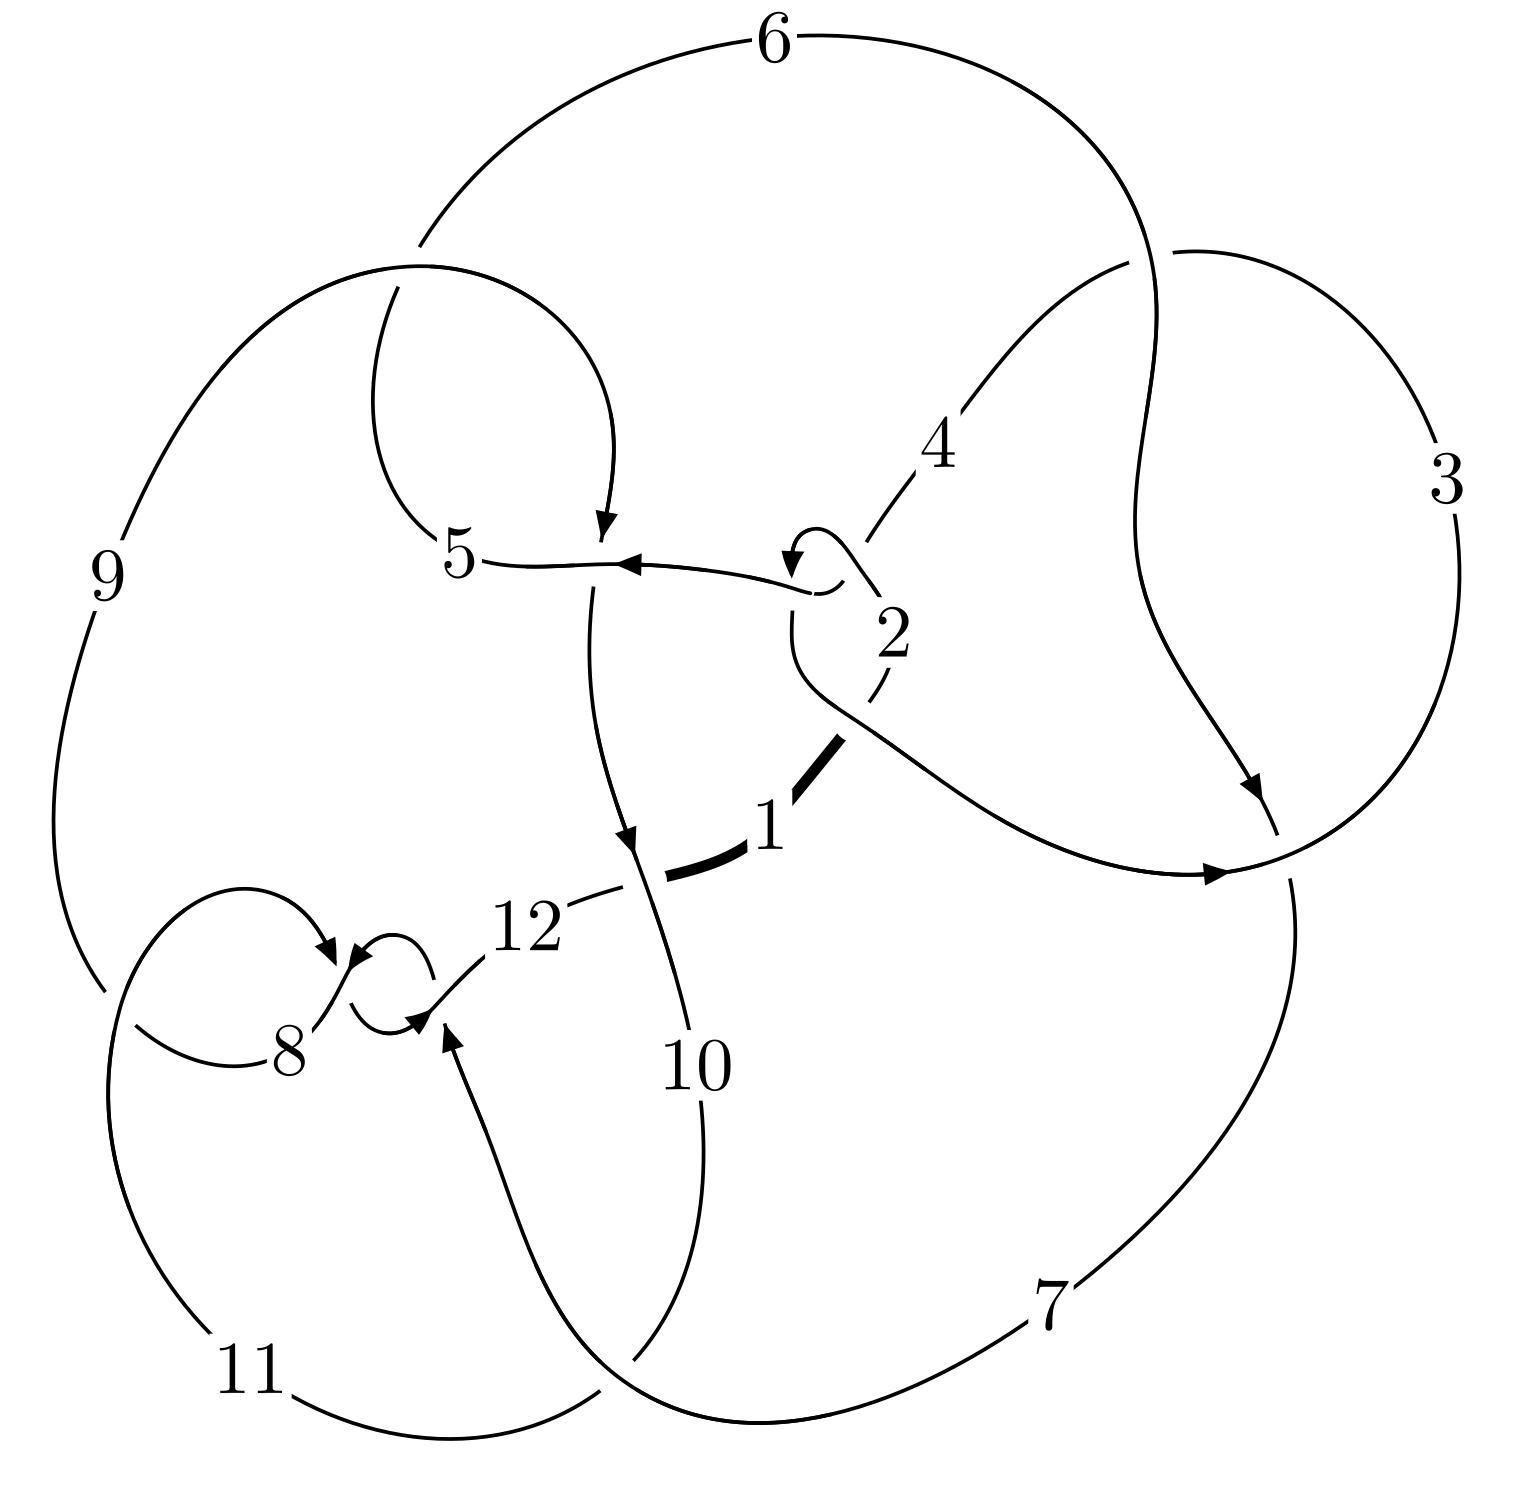
\includegraphics[width=112pt]{../../../GIT/diagram.site/Diagrams/png/2197_12n_0108.png}\\
\ \ \ A knot diagram\footnotemark}&
\allowdisplaybreaks
\textbf{Linearized knot diagam} \\
\cline{2-2}
 &
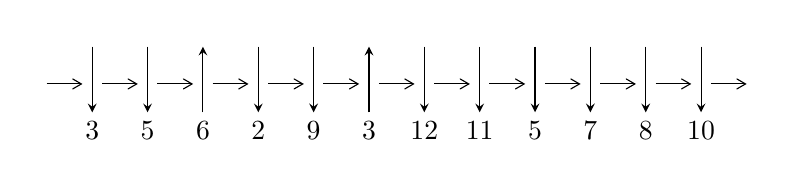
\begin{tikzpicture}[x=20pt, y=17pt]
	% nodes
	\node (C0) at (0, 0) {};
	\node (C1) at (1, 0) {};
	\node (C1U) at (1, +1) {};
	\node (C1D) at (1, -1) {3};

	\node (C2) at (2, 0) {};
	\node (C2U) at (2, +1) {};
	\node (C2D) at (2, -1) {5};

	\node (C3) at (3, 0) {};
	\node (C3U) at (3, +1) {};
	\node (C3D) at (3, -1) {6};

	\node (C4) at (4, 0) {};
	\node (C4U) at (4, +1) {};
	\node (C4D) at (4, -1) {2};

	\node (C5) at (5, 0) {};
	\node (C5U) at (5, +1) {};
	\node (C5D) at (5, -1) {9};

	\node (C6) at (6, 0) {};
	\node (C6U) at (6, +1) {};
	\node (C6D) at (6, -1) {3};

	\node (C7) at (7, 0) {};
	\node (C7U) at (7, +1) {};
	\node (C7D) at (7, -1) {12};

	\node (C8) at (8, 0) {};
	\node (C8U) at (8, +1) {};
	\node (C8D) at (8, -1) {11};

	\node (C9) at (9, 0) {};
	\node (C9U) at (9, +1) {};
	\node (C9D) at (9, -1) {5};

	\node (C10) at (10, 0) {};
	\node (C10U) at (10, +1) {};
	\node (C10D) at (10, -1) {7};

	\node (C11) at (11, 0) {};
	\node (C11U) at (11, +1) {};
	\node (C11D) at (11, -1) {8};

	\node (C12) at (12, 0) {};
	\node (C12U) at (12, +1) {};
	\node (C12D) at (12, -1) {10};
	\node (C13) at (13, 0) {};

	% arrows
	\draw[->,>={angle 60}]
	(C0) edge (C1) (C1) edge (C2) (C2) edge (C3) (C3) edge (C4) (C4) edge (C5) (C5) edge (C6) (C6) edge (C7) (C7) edge (C8) (C8) edge (C9) (C9) edge (C10) (C10) edge (C11) (C11) edge (C12) (C12) edge (C13) ;	\draw[->,>=stealth]
	(C1U) edge (C1D) (C2U) edge (C2D) (C3D) edge (C3U) (C4U) edge (C4D) (C5U) edge (C5D) (C6D) edge (C6U) (C7U) edge (C7D) (C8U) edge (C8D) (C9U) edge (C9D) (C10U) edge (C10D) (C11U) edge (C11D) (C12U) edge (C12D) ;
	\end{tikzpicture} \\
\hhline{~~} \\& 
\textbf{Solving Sequence} \\ \cline{2-2} 
 &
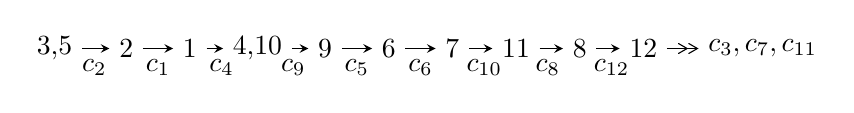
\begin{tikzpicture}[x=23pt, y=7pt]
	% node
	\node (A0) at (-1/8, 0) {3,5};
	\node (A1) at (1, 0) {2};
	\node (A2) at (2, 0) {1};
	\node (A3) at (49/16, 0) {4,10};
	\node (A4) at (33/8, 0) {9};
	\node (A5) at (41/8, 0) {6};
	\node (A6) at (49/8, 0) {7};
	\node (A7) at (57/8, 0) {11};
	\node (A8) at (65/8, 0) {8};
	\node (A9) at (73/8, 0) {12};
	\node (C1) at (1/2, -1) {$c_{2}$};
	\node (C2) at (3/2, -1) {$c_{1}$};
	\node (C3) at (5/2, -1) {$c_{4}$};
	\node (C4) at (29/8, -1) {$c_{9}$};
	\node (C5) at (37/8, -1) {$c_{5}$};
	\node (C6) at (45/8, -1) {$c_{6}$};
	\node (C7) at (53/8, -1) {$c_{10}$};
	\node (C8) at (61/8, -1) {$c_{8}$};
	\node (C9) at (69/8, -1) {$c_{12}$};
	\node (A10) at (11, 0) {$c_{3},c_{7},c_{11}$};

	% edge
	\draw[->,>=stealth]	
	(A0) edge (A1) (A1) edge (A2) (A2) edge (A3) (A3) edge (A4) (A4) edge (A5) (A5) edge (A6) (A6) edge (A7) (A7) edge (A8) (A8) edge (A9) ;
	\draw[->>,>={angle 60}]	
	(A9) edge (A10);
\end{tikzpicture} \\ 

\end{tabular} \\

\footnotetext{
The image of knot diagram is generated by the software ``\textbf{Draw programme}" developed by Andrew Bartholomew(\url{http://www.layer8.co.uk/maths/draw/index.htm\#Running-draw}), where we modified some parts for our purpose(\url{https://github.com/CATsTAILs/LinksPainter}).
}\phantom \\ \newline 
\centering \textbf{Ideals for irreducible components\footnotemark of $X_{\text{par}}$} 
 
\begin{align*}
I^u_{1}&=\langle 
-9.27106\times10^{41} u^{40}-5.88994\times10^{42} u^{39}+\cdots+9.61206\times10^{40} b-6.11993\times10^{41},\\
\phantom{I^u_{1}}&\phantom{= \langle  }-6.34476\times10^{41} u^{40}-4.08468\times10^{42} u^{39}+\cdots+9.61206\times10^{40} a-1.64646\times10^{42},\\
\phantom{I^u_{1}}&\phantom{= \langle  }u^{41}+8 u^{40}+\cdots+34 u+1\rangle \\
I^u_{2}&=\langle 
a^2+b- a+2,\;a^3+2 a+1,\;u-1\rangle \\
I^u_{3}&=\langle 
a^3- a^2+b+a-2,\;a^4- a^3+2 a^2-2 a+1,\;u-1\rangle \\
\\
\end{align*}
\raggedright * 3 irreducible components of $\dim_{\mathbb{C}}=0$, with total 48 representations.\\
\footnotetext{All coefficients of polynomials are rational numbers. But the coefficients are sometimes approximated in decimal forms when there is not enough margin.}
\newpage
\renewcommand{\arraystretch}{1}
\centering \section*{I. $I^u_{1}= \langle -9.27\times10^{41} u^{40}-5.89\times10^{42} u^{39}+\cdots+9.61\times10^{40} b-6.12\times10^{41},\;-6.34\times10^{41} u^{40}-4.08\times10^{42} u^{39}+\cdots+9.61\times10^{40} a-1.65\times10^{42},\;u^{41}+8 u^{40}+\cdots+34 u+1 \rangle$}
\flushleft \textbf{(i) Arc colorings}\\
\begin{tabular}{m{7pt} m{180pt} m{7pt} m{180pt} }
\flushright $a_{3}=$&$\begin{pmatrix}1\\0\end{pmatrix}$ \\
\flushright $a_{5}=$&$\begin{pmatrix}0\\u\end{pmatrix}$ \\
\flushright $a_{2}=$&$\begin{pmatrix}1\\- u^2\end{pmatrix}$ \\
\flushright $a_{1}=$&$\begin{pmatrix}- u^2+1\\- u^2\end{pmatrix}$ \\
\flushright $a_{4}=$&$\begin{pmatrix}u\\- u^3+u\end{pmatrix}$ \\
\flushright $a_{10}=$&$\begin{pmatrix}6.60083 u^{40}+42.4953 u^{39}+\cdots+119.918 u+17.1291\\9.64523 u^{40}+61.2765 u^{39}+\cdots+197.232 u+6.36693\end{pmatrix}$ \\
\flushright $a_{9}=$&$\begin{pmatrix}6.60083 u^{40}+42.4953 u^{39}+\cdots+119.918 u+17.1291\\-7.48281 u^{40}-47.2910 u^{39}+\cdots-146.752 u-3.94440\end{pmatrix}$ \\
\flushright $a_{6}=$&$\begin{pmatrix}-1.00706 u^{40}-6.01141 u^{39}+\cdots-9.30914 u+5.53712\\1.60537 u^{40}+9.92359 u^{39}+\cdots+28.7480 u+1.03801\end{pmatrix}$ \\
\flushright $a_{7}=$&$\begin{pmatrix}0.598315 u^{40}+3.91218 u^{39}+\cdots+19.4389 u+6.57513\\1.60537 u^{40}+9.92359 u^{39}+\cdots+28.7480 u+1.03801\end{pmatrix}$ \\
\flushright $a_{11}=$&$\begin{pmatrix}4.48614 u^{40}+28.6835 u^{39}+\cdots+68.1177 u+12.1782\\-6.77071 u^{40}-42.6663 u^{39}+\cdots-132.736 u-3.61078\end{pmatrix}$ \\
\flushright $a_{8}=$&$\begin{pmatrix}2.18696 u^{40}+13.8857 u^{39}+\cdots+34.8186 u+9.92100\\-0.720306 u^{40}-4.14288 u^{39}+\cdots-11.5196 u-0.0728726\end{pmatrix}$ \\
\flushright $a_{12}=$&$\begin{pmatrix}-0.598315 u^{40}-3.91218 u^{39}+\cdots-19.4389 u-6.57513\\1.49635 u^{40}+9.28064 u^{39}+\cdots+32.3421 u+0.715717\end{pmatrix}$\\&\end{tabular}
\flushleft \textbf{(ii) Obstruction class $= -1$}\\~\\
\flushleft \textbf{(iii) Cusp Shapes $= 8.64366 u^{40}+54.7705 u^{39}+\cdots+150.271 u-7.40030$}\\~\\
\newpage\renewcommand{\arraystretch}{1}
\flushleft \textbf{(iv) u-Polynomials at the component}\newline \\
\begin{tabular}{m{50pt}|m{274pt}}
Crossings & \hspace{64pt}u-Polynomials at each crossing \\
\hline $$\begin{aligned}c_{1}\end{aligned}$$&$\begin{aligned}
&u^{41}+50 u^{40}+\cdots+1026 u+1
\end{aligned}$\\
\hline $$\begin{aligned}c_{2},c_{4}\end{aligned}$$&$\begin{aligned}
&u^{41}-8 u^{40}+\cdots+34 u-1
\end{aligned}$\\
\hline $$\begin{aligned}c_{3},c_{6}\end{aligned}$$&$\begin{aligned}
&u^{41}+7 u^{40}+\cdots+448 u+128
\end{aligned}$\\
\hline $$\begin{aligned}c_{5},c_{9}\end{aligned}$$&$\begin{aligned}
&u^{41}+2 u^{40}+\cdots- u-1
\end{aligned}$\\
\hline $$\begin{aligned}c_{7},c_{8},c_{11}\end{aligned}$$&$\begin{aligned}
&u^{41}-2 u^{40}+\cdots-3 u-1
\end{aligned}$\\
\hline $$\begin{aligned}c_{10}\end{aligned}$$&$\begin{aligned}
&u^{41}+2 u^{40}+\cdots-240 u-36
\end{aligned}$\\
\hline $$\begin{aligned}c_{12}\end{aligned}$$&$\begin{aligned}
&u^{41}-12 u^{40}+\cdots-467 u+163
\end{aligned}$\\
\hline
\end{tabular}\\~\\
\newpage\renewcommand{\arraystretch}{1}
\flushleft \textbf{(v) Riley Polynomials at the component}\newline \\
\begin{tabular}{m{50pt}|m{274pt}}
Crossings & \hspace{64pt}Riley Polynomials at each crossing \\
\hline $$\begin{aligned}c_{1}\end{aligned}$$&$\begin{aligned}
&y^{41}-110 y^{40}+\cdots+1177934 y-1
\end{aligned}$\\
\hline $$\begin{aligned}c_{2},c_{4}\end{aligned}$$&$\begin{aligned}
&y^{41}-50 y^{40}+\cdots+1026 y-1
\end{aligned}$\\
\hline $$\begin{aligned}c_{3},c_{6}\end{aligned}$$&$\begin{aligned}
&y^{41}+45 y^{40}+\cdots+520192 y-16384
\end{aligned}$\\
\hline $$\begin{aligned}c_{5},c_{9}\end{aligned}$$&$\begin{aligned}
&y^{41}+42 y^{39}+\cdots+11 y-1
\end{aligned}$\\
\hline $$\begin{aligned}c_{7},c_{8},c_{11}\end{aligned}$$&$\begin{aligned}
&y^{41}+36 y^{40}+\cdots+11 y-1
\end{aligned}$\\
\hline $$\begin{aligned}c_{10}\end{aligned}$$&$\begin{aligned}
&y^{41}-12 y^{40}+\cdots+7992 y-1296
\end{aligned}$\\
\hline $$\begin{aligned}c_{12}\end{aligned}$$&$\begin{aligned}
&y^{41}-12 y^{40}+\cdots+2120951 y-26569
\end{aligned}$\\
\hline
\end{tabular}\\~\\
\newpage\flushleft \textbf{(vi) Complex Volumes and Cusp Shapes}
$$\begin{array}{c|c|c}  
\text{Solutions to }I^u_{1}& \I (\text{vol} + \sqrt{-1}CS) & \text{Cusp shape}\\
 \hline 
\begin{aligned}
u &= \phantom{-}1.023890 + 0.144827 I \\
a &= -0.114598 + 0.492587 I \\
b &= -0.25937 - 2.41362 I\end{aligned}
 & \phantom{-}1.10253 + 2.40302 I & -1.4441 - 16.6541 I \\ \hline\begin{aligned}
u &= \phantom{-}1.023890 - 0.144827 I \\
a &= -0.114598 - 0.492587 I \\
b &= -0.25937 + 2.41362 I\end{aligned}
 & \phantom{-}1.10253 - 2.40302 I & -1.4441 + 16.6541 I \\ \hline\begin{aligned}
u &= \phantom{-}1.09654\phantom{ +0.000000I} \\
a &= \phantom{-}0.432301\phantom{ +0.000000I} \\
b &= \phantom{-}1.83917\phantom{ +0.000000I}\end{aligned}
 & -2.21383\phantom{ +0.000000I} & \phantom{-}3.32100\phantom{ +0.000000I} \\ \hline\begin{aligned}
u &= \phantom{-}0.799614 + 0.163499 I \\
a &= \phantom{-}0.305351 - 0.647956 I \\
b &= \phantom{-}0.24502 + 1.73105 I\end{aligned}
 & -2.56053 - 0.52413 I & -15.2569 - 4.2496 I \\ \hline\begin{aligned}
u &= \phantom{-}0.799614 - 0.163499 I \\
a &= \phantom{-}0.305351 + 0.647956 I \\
b &= \phantom{-}0.24502 - 1.73105 I\end{aligned}
 & -2.56053 + 0.52413 I & -15.2569 + 4.2496 I \\ \hline\begin{aligned}
u &= \phantom{-}0.618990 + 0.472493 I \\
a &= -0.934348 - 0.002226 I \\
b &= -0.492958 + 0.445400 I\end{aligned}
 & -0.79846 - 1.42488 I & -6.70258 + 4.89942 I \\ \hline\begin{aligned}
u &= \phantom{-}0.618990 - 0.472493 I \\
a &= -0.934348 + 0.002226 I \\
b &= -0.492958 - 0.445400 I\end{aligned}
 & -0.79846 + 1.42488 I & -6.70258 - 4.89942 I \\ \hline\begin{aligned}
u &= \phantom{-}0.654305 + 0.324584 I \\
a &= -0.185932 + 0.902814 I \\
b &= \phantom{-}0.19586 - 1.59294 I\end{aligned}
 & \phantom{-}1.89593 - 3.76450 I & -6.51510 - 0.37648 I \\ \hline\begin{aligned}
u &= \phantom{-}0.654305 - 0.324584 I \\
a &= -0.185932 - 0.902814 I \\
b &= \phantom{-}0.19586 + 1.59294 I\end{aligned}
 & \phantom{-}1.89593 + 3.76450 I & -6.51510 + 0.37648 I \\ \hline\begin{aligned}
u &= \phantom{-}0.024088 + 0.729003 I \\
a &= \phantom{-}0.975104 - 0.793348 I \\
b &= \phantom{-}0.015225 - 0.189698 I\end{aligned}
 & \phantom{-}4.22621 - 1.38545 I & -1.96542 + 3.48117 I\\
 \hline 
 \end{array}$$\newpage$$\begin{array}{c|c|c}  
\text{Solutions to }I^u_{1}& \I (\text{vol} + \sqrt{-1}CS) & \text{Cusp shape}\\
 \hline 
\begin{aligned}
u &= \phantom{-}0.024088 - 0.729003 I \\
a &= \phantom{-}0.975104 + 0.793348 I \\
b &= \phantom{-}0.015225 + 0.189698 I\end{aligned}
 & \phantom{-}4.22621 + 1.38545 I & -1.96542 - 3.48117 I \\ \hline\begin{aligned}
u &= -0.690147 + 0.145492 I \\
a &= \phantom{-}0.04771 - 1.93802 I \\
b &= -0.236345 - 0.828778 I\end{aligned}
 & \phantom{-}8.34723 - 4.89832 I & \phantom{-}3.94388 + 1.15377 I \\ \hline\begin{aligned}
u &= -0.690147 - 0.145492 I \\
a &= \phantom{-}0.04771 + 1.93802 I \\
b &= -0.236345 + 0.828778 I\end{aligned}
 & \phantom{-}8.34723 + 4.89832 I & \phantom{-}3.94388 - 1.15377 I \\ \hline\begin{aligned}
u &= \phantom{-}0.784586 + 1.118630 I \\
a &= \phantom{-}0.619859 - 0.276128 I \\
b &= \phantom{-}0.550920 + 0.122912 I\end{aligned}
 & -3.61696 - 3.86307 I & \phantom{-0.000000 } 0 \\ \hline\begin{aligned}
u &= \phantom{-}0.784586 - 1.118630 I \\
a &= \phantom{-}0.619859 + 0.276128 I \\
b &= \phantom{-}0.550920 - 0.122912 I\end{aligned}
 & -3.61696 + 3.86307 I & \phantom{-0.000000 } 0 \\ \hline\begin{aligned}
u &= \phantom{-}1.06503 + 0.93172 I \\
a &= -0.595278 + 0.164576 I \\
b &= -0.773274 - 0.052105 I\end{aligned}
 & -0.499621 - 0.427314 I & \phantom{-0.000000 } 0 \\ \hline\begin{aligned}
u &= \phantom{-}1.06503 - 0.93172 I \\
a &= -0.595278 - 0.164576 I \\
b &= -0.773274 + 0.052105 I\end{aligned}
 & -0.499621 + 0.427314 I & \phantom{-0.000000 } 0 \\ \hline\begin{aligned}
u &= \phantom{-}0.64097 + 1.26233 I \\
a &= -0.593984 + 0.346167 I \\
b &= -0.439012 - 0.204480 I\end{aligned}
 & \phantom{-}0.95653 - 7.53305 I & \phantom{-0.000000 } 0 \\ \hline\begin{aligned}
u &= \phantom{-}0.64097 - 1.26233 I \\
a &= -0.593984 - 0.346167 I \\
b &= -0.439012 + 0.204480 I\end{aligned}
 & \phantom{-}0.95653 + 7.53305 I & \phantom{-0.000000 } 0 \\ \hline\begin{aligned}
u &= -0.546543 + 0.110125 I \\
a &= -0.15010 + 2.08713 I \\
b &= \phantom{-}0.113534 + 0.680577 I\end{aligned}
 & \phantom{-}2.42231 - 1.86356 I & -0.33827 + 3.07051 I\\
 \hline 
 \end{array}$$\newpage$$\begin{array}{c|c|c}  
\text{Solutions to }I^u_{1}& \I (\text{vol} + \sqrt{-1}CS) & \text{Cusp shape}\\
 \hline 
\begin{aligned}
u &= -0.546543 - 0.110125 I \\
a &= -0.15010 - 2.08713 I \\
b &= \phantom{-}0.113534 - 0.680577 I\end{aligned}
 & \phantom{-}2.42231 + 1.86356 I & -0.33827 - 3.07051 I \\ \hline\begin{aligned}
u &= -1.52433 + 0.18776 I \\
a &= -0.857605 + 0.620146 I \\
b &= -1.95651 + 0.55267 I\end{aligned}
 & -1.30698 + 4.28669 I & \phantom{-0.000000 } 0 \\ \hline\begin{aligned}
u &= -1.52433 - 0.18776 I \\
a &= -0.857605 - 0.620146 I \\
b &= -1.95651 - 0.55267 I\end{aligned}
 & -1.30698 - 4.28669 I & \phantom{-0.000000 } 0 \\ \hline\begin{aligned}
u &= -1.64128 + 0.09999 I \\
a &= \phantom{-}0.638107 + 0.741558 I \\
b &= \phantom{-}1.78817 + 0.37849 I\end{aligned}
 & -6.19266 + 5.42860 I & \phantom{-0.000000 } 0 \\ \hline\begin{aligned}
u &= -1.64128 - 0.09999 I \\
a &= \phantom{-}0.638107 - 0.741558 I \\
b &= \phantom{-}1.78817 - 0.37849 I\end{aligned}
 & -6.19266 - 5.42860 I & \phantom{-0.000000 } 0 \\ \hline\begin{aligned}
u &= -1.68045 + 0.02735 I \\
a &= -0.661327 - 0.687909 I \\
b &= -1.85642 - 0.38244 I\end{aligned}
 & -11.48150 + 1.16744 I & \phantom{-0.000000 } 0 \\ \hline\begin{aligned}
u &= -1.68045 - 0.02735 I \\
a &= -0.661327 + 0.687909 I \\
b &= -1.85642 + 0.38244 I\end{aligned}
 & -11.48150 - 1.16744 I & \phantom{-0.000000 } 0 \\ \hline\begin{aligned}
u &= -1.68637 + 0.08037 I \\
a &= \phantom{-}0.707793 - 0.630890 I \\
b &= \phantom{-}1.93021 - 0.41903 I\end{aligned}
 & -9.39900 + 3.48257 I & \phantom{-0.000000 } 0 \\ \hline\begin{aligned}
u &= -1.68637 - 0.08037 I \\
a &= \phantom{-}0.707793 + 0.630890 I \\
b &= \phantom{-}1.93021 + 0.41903 I\end{aligned}
 & -9.39900 - 3.48257 I & \phantom{-0.000000 } 0 \\ \hline\begin{aligned}
u &= -1.69925 + 0.27352 I \\
a &= \phantom{-}0.758442 - 0.516353 I \\
b &= \phantom{-}2.04847 - 0.47151 I\end{aligned}
 & -9.49392 + 4.85059 I & \phantom{-0.000000 } 0\\
 \hline 
 \end{array}$$\newpage$$\begin{array}{c|c|c}  
\text{Solutions to }I^u_{1}& \I (\text{vol} + \sqrt{-1}CS) & \text{Cusp shape}\\
 \hline 
\begin{aligned}
u &= -1.69925 - 0.27352 I \\
a &= \phantom{-}0.758442 + 0.516353 I \\
b &= \phantom{-}2.04847 + 0.47151 I\end{aligned}
 & -9.49392 - 4.85059 I & \phantom{-0.000000 } 0 \\ \hline\begin{aligned}
u &= -1.67351 + 0.43283 I \\
a &= \phantom{-}0.792521 - 0.425685 I \\
b &= \phantom{-}2.12131 - 0.52943 I\end{aligned}
 & -6.4546 + 13.6928 I & \phantom{-0.000000 } 0 \\ \hline\begin{aligned}
u &= -1.67351 - 0.43283 I \\
a &= \phantom{-}0.792521 + 0.425685 I \\
b &= \phantom{-}2.12131 + 0.52943 I\end{aligned}
 & -6.4546 - 13.6928 I & \phantom{-0.000000 } 0 \\ \hline\begin{aligned}
u &= -1.70062 + 0.36989 I \\
a &= -0.772140 + 0.460082 I \\
b &= -2.09871 + 0.49854 I\end{aligned}
 & -11.6676 + 9.4552 I & \phantom{-0.000000 } 0 \\ \hline\begin{aligned}
u &= -1.70062 - 0.36989 I \\
a &= -0.772140 - 0.460082 I \\
b &= -2.09871 - 0.49854 I\end{aligned}
 & -11.6676 - 9.4552 I & \phantom{-0.000000 } 0 \\ \hline\begin{aligned}
u &= \phantom{-}1.79083\phantom{ +0.000000I} \\
a &= -0.471299\phantom{ +0.000000I} \\
b &= -1.27778\phantom{ +0.000000I}\end{aligned}
 & -5.96639\phantom{ +0.000000I} & \phantom{-0.000000 } 0 \\ \hline\begin{aligned}
u &= \phantom{-}1.80924 + 0.21929 I \\
a &= \phantom{-}0.470409 - 0.020609 I \\
b &= \phantom{-}1.266140 + 0.027083 I\end{aligned}
 & -2.04881 - 3.64658 I & \phantom{-0.000000 } 0 \\ \hline\begin{aligned}
u &= \phantom{-}1.80924 - 0.21929 I \\
a &= \phantom{-}0.470409 + 0.020609 I \\
b &= \phantom{-}1.266140 - 0.027083 I\end{aligned}
 & -2.04881 + 3.64658 I & \phantom{-0.000000 } 0 \\ \hline\begin{aligned}
u &= -0.006712 + 0.160531 I \\
a &= -1.90793 - 3.46251 I \\
b &= -0.690720 + 0.504582 I\end{aligned}
 & \phantom{-}3.36845 + 2.26324 I & -4.13576 - 3.78467 I \\ \hline\begin{aligned}
u &= -0.006712 - 0.160531 I \\
a &= -1.90793 + 3.46251 I \\
b &= -0.690720 - 0.504582 I\end{aligned}
 & \phantom{-}3.36845 - 2.26324 I & -4.13576 + 3.78467 I\\
 \hline 
 \end{array}$$\newpage$$\begin{array}{c|c|c}  
\text{Solutions to }I^u_{1}& \I (\text{vol} + \sqrt{-1}CS) & \text{Cusp shape}\\
 \hline 
\begin{aligned}
u &= -0.0303735\phantom{ +0.000000I} \\
a &= \phantom{-}13.9549\phantom{ +0.000000I} \\
b &= \phantom{-}0.495519\phantom{ +0.000000I}\end{aligned}
 & -0.822843\phantom{ +0.000000I} & -12.1130\phantom{ +0.000000I}\\
 \hline 
 \end{array}$$\newpage\newpage\renewcommand{\arraystretch}{1}
\centering \section*{II. $I^u_{2}= \langle a^2+b- a+2,\;a^3+2 a+1,\;u-1 \rangle$}
\flushleft \textbf{(i) Arc colorings}\\
\begin{tabular}{m{7pt} m{180pt} m{7pt} m{180pt} }
\flushright $a_{3}=$&$\begin{pmatrix}1\\0\end{pmatrix}$ \\
\flushright $a_{5}=$&$\begin{pmatrix}0\\1\end{pmatrix}$ \\
\flushright $a_{2}=$&$\begin{pmatrix}1\\-1\end{pmatrix}$ \\
\flushright $a_{1}=$&$\begin{pmatrix}0\\-1\end{pmatrix}$ \\
\flushright $a_{4}=$&$\begin{pmatrix}1\\0\end{pmatrix}$ \\
\flushright $a_{10}=$&$\begin{pmatrix}a\\- a^2+a-2\end{pmatrix}$ \\
\flushright $a_{9}=$&$\begin{pmatrix}a\\- a^2-2\end{pmatrix}$ \\
\flushright $a_{6}=$&$\begin{pmatrix}- a^2\\0\end{pmatrix}$ \\
\flushright $a_{7}=$&$\begin{pmatrix}- a^2\\0\end{pmatrix}$ \\
\flushright $a_{11}=$&$\begin{pmatrix}a^2- a-1\\- a^2+a-2\end{pmatrix}$ \\
\flushright $a_{8}=$&$\begin{pmatrix}- a^2-2 a-1\\-1\end{pmatrix}$ \\
\flushright $a_{12}=$&$\begin{pmatrix}- a^2\\- a^2-2\end{pmatrix}$\\&\end{tabular}
\flushleft \textbf{(ii) Obstruction class $= 1$}\\~\\
\flushleft \textbf{(iii) Cusp Shapes $= -11 a^2+9 a-34$}\\~\\
\newpage\renewcommand{\arraystretch}{1}
\flushleft \textbf{(iv) u-Polynomials at the component}\newline \\
\begin{tabular}{m{50pt}|m{274pt}}
Crossings & \hspace{64pt}u-Polynomials at each crossing \\
\hline $$\begin{aligned}c_{1},c_{2}\end{aligned}$$&$\begin{aligned}
&(u-1)^3
\end{aligned}$\\
\hline $$\begin{aligned}c_{3},c_{6}\end{aligned}$$&$\begin{aligned}
&u^3
\end{aligned}$\\
\hline $$\begin{aligned}c_{4}\end{aligned}$$&$\begin{aligned}
&(u+1)^3
\end{aligned}$\\
\hline $$\begin{aligned}c_{5},c_{7},c_{8}\end{aligned}$$&$\begin{aligned}
&u^3+2 u-1
\end{aligned}$\\
\hline $$\begin{aligned}c_{9},c_{11},c_{12}\end{aligned}$$&$\begin{aligned}
&u^3+2 u+1
\end{aligned}$\\
\hline $$\begin{aligned}c_{10}\end{aligned}$$&$\begin{aligned}
&u^3+3 u^2+5 u+2
\end{aligned}$\\
\hline
\end{tabular}\\~\\
\newpage\renewcommand{\arraystretch}{1}
\flushleft \textbf{(v) Riley Polynomials at the component}\newline \\
\begin{tabular}{m{50pt}|m{274pt}}
Crossings & \hspace{64pt}Riley Polynomials at each crossing \\
\hline $$\begin{aligned}c_{1},c_{2},c_{4}\end{aligned}$$&$\begin{aligned}
&(y-1)^3
\end{aligned}$\\
\hline $$\begin{aligned}c_{3},c_{6}\end{aligned}$$&$\begin{aligned}
&y^3
\end{aligned}$\\
\hline $$\begin{aligned}c_{5},c_{7},c_{8}\\c_{9},c_{11},c_{12}\end{aligned}$$&$\begin{aligned}
&y^3+4 y^2+4 y-1
\end{aligned}$\\
\hline $$\begin{aligned}c_{10}\end{aligned}$$&$\begin{aligned}
&y^3+y^2+13 y-4
\end{aligned}$\\
\hline
\end{tabular}\\~\\
\newpage\flushleft \textbf{(vi) Complex Volumes and Cusp Shapes}
$$\begin{array}{c|c|c}  
\text{Solutions to }I^u_{2}& \I (\text{vol} + \sqrt{-1}CS) & \text{Cusp shape}\\
 \hline 
\begin{aligned}
u &= \phantom{-}1.00000\phantom{ +0.000000I} \\
a &= \phantom{-}0.22670 + 1.46771 I \\
b &= \phantom{-}0.329484 + 0.802255 I\end{aligned}
 & \phantom{-}7.79580 - 5.13794 I & -8.82908 + 5.88938 I \\ \hline\begin{aligned}
u &= \phantom{-}1.00000\phantom{ +0.000000I} \\
a &= \phantom{-}0.22670 - 1.46771 I \\
b &= \phantom{-}0.329484 - 0.802255 I\end{aligned}
 & \phantom{-}7.79580 + 5.13794 I & -8.82908 - 5.88938 I \\ \hline\begin{aligned}
u &= \phantom{-}1.00000\phantom{ +0.000000I} \\
a &= -0.453398\phantom{ +0.000000I} \\
b &= -2.65897\phantom{ +0.000000I}\end{aligned}
 & -2.43213\phantom{ +0.000000I} & -40.3420\phantom{ +0.000000I}\\
 \hline 
 \end{array}$$\newpage\newpage\renewcommand{\arraystretch}{1}
\centering \section*{III. $I^u_{3}= \langle a^3- a^2+b+a-2,\;a^4- a^3+2 a^2-2 a+1,\;u-1 \rangle$}
\flushleft \textbf{(i) Arc colorings}\\
\begin{tabular}{m{7pt} m{180pt} m{7pt} m{180pt} }
\flushright $a_{3}=$&$\begin{pmatrix}1\\0\end{pmatrix}$ \\
\flushright $a_{5}=$&$\begin{pmatrix}0\\1\end{pmatrix}$ \\
\flushright $a_{2}=$&$\begin{pmatrix}1\\-1\end{pmatrix}$ \\
\flushright $a_{1}=$&$\begin{pmatrix}0\\-1\end{pmatrix}$ \\
\flushright $a_{4}=$&$\begin{pmatrix}1\\0\end{pmatrix}$ \\
\flushright $a_{10}=$&$\begin{pmatrix}a\\- a^3+a^2- a+2\end{pmatrix}$ \\
\flushright $a_{9}=$&$\begin{pmatrix}a\\- a^3+a^2-2 a+2\end{pmatrix}$ \\
\flushright $a_{6}=$&$\begin{pmatrix}- a^2\\0\end{pmatrix}$ \\
\flushright $a_{7}=$&$\begin{pmatrix}- a^2\\0\end{pmatrix}$ \\
\flushright $a_{11}=$&$\begin{pmatrix}1\\- a^3+a^2- a+2\end{pmatrix}$ \\
\flushright $a_{8}=$&$\begin{pmatrix}- a^3- a+1\\-3 a^3+a^2-5 a+3\end{pmatrix}$ \\
\flushright $a_{12}=$&$\begin{pmatrix}- a^2\\- a^2-2\end{pmatrix}$\\&\end{tabular}
\flushleft \textbf{(ii) Obstruction class $= 1$}\\~\\
\flushleft \textbf{(iii) Cusp Shapes $= 4 a^3+3 a^2+4 a-8$}\\~\\
\newpage\renewcommand{\arraystretch}{1}
\flushleft \textbf{(iv) u-Polynomials at the component}\newline \\
\begin{tabular}{m{50pt}|m{274pt}}
Crossings & \hspace{64pt}u-Polynomials at each crossing \\
\hline $$\begin{aligned}c_{1},c_{2}\end{aligned}$$&$\begin{aligned}
&(u-1)^4
\end{aligned}$\\
\hline $$\begin{aligned}c_{3},c_{6}\end{aligned}$$&$\begin{aligned}
&u^4
\end{aligned}$\\
\hline $$\begin{aligned}c_{4}\end{aligned}$$&$\begin{aligned}
&(u+1)^4
\end{aligned}$\\
\hline $$\begin{aligned}c_{5},c_{7},c_{8}\end{aligned}$$&$\begin{aligned}
&u^4+u^3+2 u^2+2 u+1
\end{aligned}$\\
\hline $$\begin{aligned}c_{9},c_{11},c_{12}\end{aligned}$$&$\begin{aligned}
&u^4- u^3+2 u^2-2 u+1
\end{aligned}$\\
\hline $$\begin{aligned}c_{10}\end{aligned}$$&$\begin{aligned}
&(u^2- u+1)^2
\end{aligned}$\\
\hline
\end{tabular}\\~\\
\newpage\renewcommand{\arraystretch}{1}
\flushleft \textbf{(v) Riley Polynomials at the component}\newline \\
\begin{tabular}{m{50pt}|m{274pt}}
Crossings & \hspace{64pt}Riley Polynomials at each crossing \\
\hline $$\begin{aligned}c_{1},c_{2},c_{4}\end{aligned}$$&$\begin{aligned}
&(y-1)^4
\end{aligned}$\\
\hline $$\begin{aligned}c_{3},c_{6}\end{aligned}$$&$\begin{aligned}
&y^4
\end{aligned}$\\
\hline $$\begin{aligned}c_{5},c_{7},c_{8}\\c_{9},c_{11},c_{12}\end{aligned}$$&$\begin{aligned}
&y^4+3 y^3+2 y^2+1
\end{aligned}$\\
\hline $$\begin{aligned}c_{10}\end{aligned}$$&$\begin{aligned}
&(y^2+y+1)^2
\end{aligned}$\\
\hline
\end{tabular}\\~\\
\newpage\flushleft \textbf{(vi) Complex Volumes and Cusp Shapes}
$$\begin{array}{c|c|c}  
\text{Solutions to }I^u_{3}& \I (\text{vol} + \sqrt{-1}CS) & \text{Cusp shape}\\
 \hline 
\begin{aligned}
u &= \phantom{-}1.00000\phantom{ +0.000000I} \\
a &= \phantom{-}0.621744 + 0.440597 I \\
b &= \phantom{-}1.69244 - 0.31815 I\end{aligned}
 & \phantom{-}1.64493 - 2.02988 I & -5.42268 + 5.10773 I \\ \hline\begin{aligned}
u &= \phantom{-}1.00000\phantom{ +0.000000I} \\
a &= \phantom{-}0.621744 - 0.440597 I \\
b &= \phantom{-}1.69244 + 0.31815 I\end{aligned}
 & \phantom{-}1.64493 + 2.02988 I & -5.42268 - 5.10773 I \\ \hline\begin{aligned}
u &= \phantom{-}1.00000\phantom{ +0.000000I} \\
a &= -0.121744 + 1.306620 I \\
b &= -0.192440 + 0.547877 I\end{aligned}
 & \phantom{-}1.64493 + 2.02988 I & -11.07732 - 4.41855 I \\ \hline\begin{aligned}
u &= \phantom{-}1.00000\phantom{ +0.000000I} \\
a &= -0.121744 - 1.306620 I \\
b &= -0.192440 - 0.547877 I\end{aligned}
 & \phantom{-}1.64493 - 2.02988 I & -11.07732 + 4.41855 I\\
 \hline 
 \end{array}$$\newpage
\newpage\renewcommand{\arraystretch}{1}
\centering \section*{ IV. u-Polynomials}
\begin{tabular}{m{50pt}|m{274pt}}
Crossings & \hspace{64pt}u-Polynomials at each crossing \\
\hline $$\begin{aligned}c_{1}\end{aligned}$$&$\begin{aligned}
&((u-1)^7)(u^{41}+50 u^{40}+\cdots+1026 u+1)
\end{aligned}$\\
\hline $$\begin{aligned}c_{2}\end{aligned}$$&$\begin{aligned}
&((u-1)^7)(u^{41}-8 u^{40}+\cdots+34 u-1)
\end{aligned}$\\
\hline $$\begin{aligned}c_{3},c_{6}\end{aligned}$$&$\begin{aligned}
&u^7(u^{41}+7 u^{40}+\cdots+448 u+128)
\end{aligned}$\\
\hline $$\begin{aligned}c_{4}\end{aligned}$$&$\begin{aligned}
&((u+1)^7)(u^{41}-8 u^{40}+\cdots+34 u-1)
\end{aligned}$\\
\hline $$\begin{aligned}c_{5}\end{aligned}$$&$\begin{aligned}
&(u^3+2 u-1)(u^4+u^3+2 u^2+2 u+1)(u^{41}+2 u^{40}+\cdots- u-1)
\end{aligned}$\\
\hline $$\begin{aligned}c_{7},c_{8}\end{aligned}$$&$\begin{aligned}
&(u^3+2 u-1)(u^4+u^3+2 u^2+2 u+1)(u^{41}-2 u^{40}+\cdots-3 u-1)
\end{aligned}$\\
\hline $$\begin{aligned}c_{9}\end{aligned}$$&$\begin{aligned}
&(u^3+2 u+1)(u^4- u^3+2 u^2-2 u+1)(u^{41}+2 u^{40}+\cdots- u-1)
\end{aligned}$\\
\hline $$\begin{aligned}c_{10}\end{aligned}$$&$\begin{aligned}
&((u^2- u+1)^2)(u^3+3 u^2+5 u+2)(u^{41}+2 u^{40}+\cdots-240 u-36)
\end{aligned}$\\
\hline $$\begin{aligned}c_{11}\end{aligned}$$&$\begin{aligned}
&(u^3+2 u+1)(u^4- u^3+2 u^2-2 u+1)(u^{41}-2 u^{40}+\cdots-3 u-1)
\end{aligned}$\\
\hline $$\begin{aligned}c_{12}\end{aligned}$$&$\begin{aligned}
&(u^3+2 u+1)(u^4- u^3+2 u^2-2 u+1)(u^{41}-12 u^{40}+\cdots-467 u+163)
\end{aligned}$\\
\hline
\end{tabular}\newpage\renewcommand{\arraystretch}{1}
\centering \section*{ V. Riley Polynomials}
\begin{tabular}{m{50pt}|m{274pt}}
Crossings & \hspace{64pt}Riley Polynomials at each crossing \\
\hline $$\begin{aligned}c_{1}\end{aligned}$$&$\begin{aligned}
&((y-1)^7)(y^{41}-110 y^{40}+\cdots+1177934 y-1)
\end{aligned}$\\
\hline $$\begin{aligned}c_{2},c_{4}\end{aligned}$$&$\begin{aligned}
&((y-1)^7)(y^{41}-50 y^{40}+\cdots+1026 y-1)
\end{aligned}$\\
\hline $$\begin{aligned}c_{3},c_{6}\end{aligned}$$&$\begin{aligned}
&y^7(y^{41}+45 y^{40}+\cdots+520192 y-16384)
\end{aligned}$\\
\hline $$\begin{aligned}c_{5},c_{9}\end{aligned}$$&$\begin{aligned}
&(y^3+4 y^2+4 y-1)(y^4+3 y^3+2 y^2+1)(y^{41}+42 y^{39}+\cdots+11 y-1)
\end{aligned}$\\
\hline $$\begin{aligned}c_{7},c_{8},c_{11}\end{aligned}$$&$\begin{aligned}
&(y^3+4 y^2+4 y-1)(y^4+3 y^3+2 y^2+1)(y^{41}+36 y^{40}+\cdots+11 y-1)
\end{aligned}$\\
\hline $$\begin{aligned}c_{10}\end{aligned}$$&$\begin{aligned}
&((y^2+y+1)^2)(y^3+y^2+13 y-4)(y^{41}-12 y^{40}+\cdots+7992 y-1296)
\end{aligned}$\\
\hline $$\begin{aligned}c_{12}\end{aligned}$$&$\begin{aligned}
&(y^3+4 y^2+4 y-1)(y^4+3 y^3+2 y^2+1)\\
&\cdot(y^{41}-12 y^{40}+\cdots+2120951 y-26569)
\end{aligned}$\\
\hline
\end{tabular}
\vskip 2pc
\end{document}